\documentclass{../../zirkelblatt}

\usepackage{geometry}
\geometry{tmargin=0.5cm,bmargin=0.5cm,lmargin=1cm,rmargin=1cm}

\pagestyle{empty}

\newcommand{\ppp}{\mathfrak{p}}
\newcommand{\qqq}{\mathfrak{q}}

\begin{document}

\newcommand{\vorderseite}{
  \begin{minipage}[t][4cm][t]{7.6cm}
    \begin{center}
      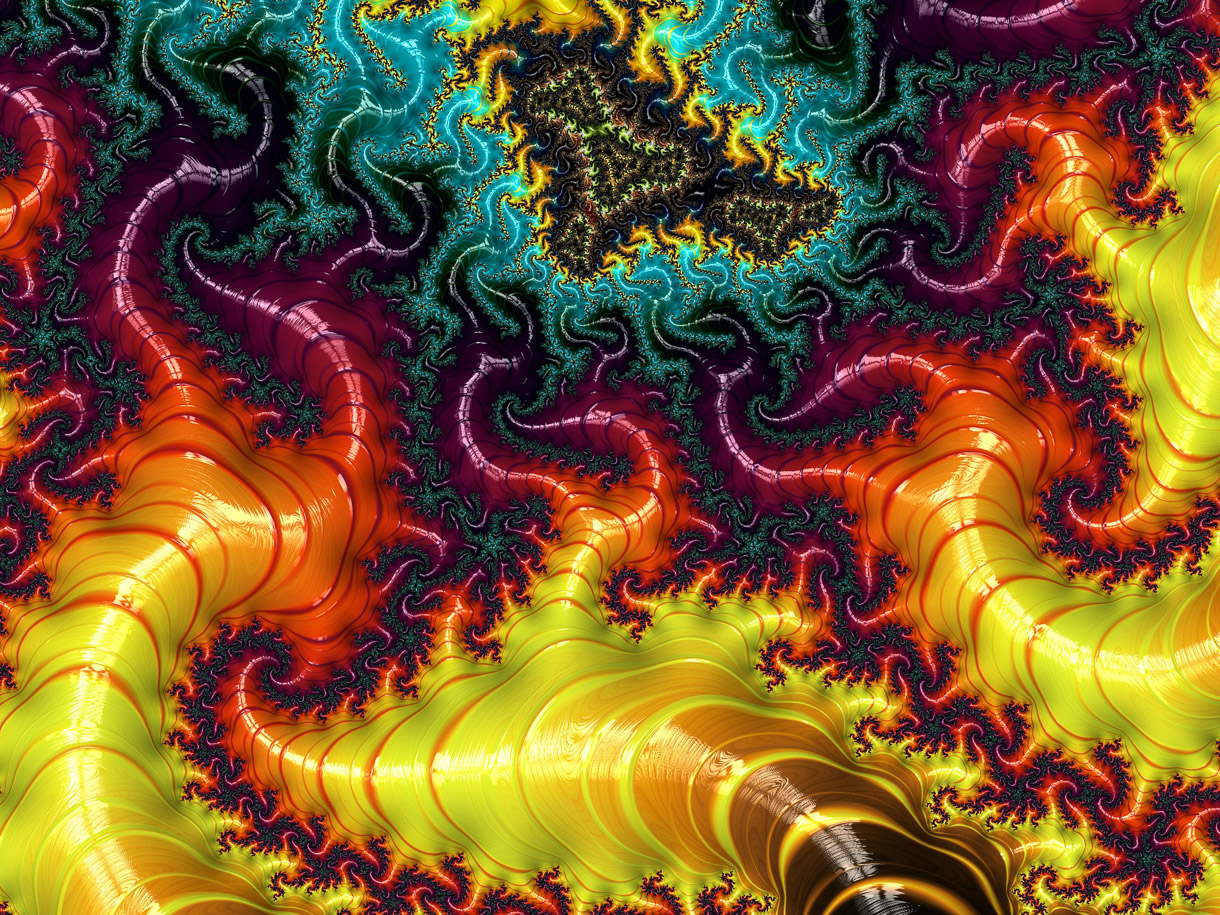
\includegraphics[width=0.8\textwidth,height=4cm]{fractal}
    \end{center}
  \end{minipage}
}

\newcommand{\rueckseite}{
  \begin{minipage}[t][4cm][t]{7.6cm}
    \phantom{A}
    \vspace{-0.3em}
    \tiny

    \textbf{Über die Unmöglichkeit der universellen Lokalisierung in der
    Kategorie der Mengen.} Sei~$A$ ein kommutativer Ring. Sei~$\alpha : A \to
    A'$ eine hypothetische universelle Lokalisierung von~$A$, also ein
    lokaler Ring mit der Eigenschaft, dass jeder Ringhomomorphismus~$A \to B$
    in einen lokalen Ring auf eindeutige Art und Weise Komposition von~$\alpha$
    mit einem lokalen Ringhomomorphismus~$A' \to B$ ist. Dann sind je zwei
    Primideale von~$A$ gleich: Seien~$\ppp$ und~$\qqq$ Primideale. Sei~$s
    \not\in \ppp$ beliebig. Da~$s$ unter dem Ringhomo~$A \to A_\ppp$ auf ein
    invertierbares Element geschickt wird und~$A' \to A_\ppp$ lokal ist,
    ist~$\alpha(s)$ in~$A'$ invertierbar. Somit ist auch das Bild von~$s$
    unter~$A \to A_\qqq$ invertierbar. Also~$s \not\in \qqq$.
    \medskip

    \textbf{Das Optimierungsproblem besitzt nur dann eine Lösung,} wenn man
    bereit ist, den Topos zu wechseln. Die Lösung ist dann die Strukturgarbe im
    Topos der Garben auf dem Spektrum von~$A$. Diese kann man als Lokalisierung der
    konstanten Garbe~$\underline{A}$ an dem \textbf{universellen Filter}
    konstruieren, wobei der universelle Filter die Garbe der lokal konstanten
    Funktionen~$f : U \to A$ mit $f(\ppp) \not\in \ppp$ für alle~$\ppp \in U$
    ist.
  \end{minipage}
}

\vorderseite\hfill\vorderseite
\vfill
\vorderseite\hfill\vorderseite
\vfill
\vorderseite\hfill\vorderseite
\vfill
\vorderseite\hfill\vorderseite
\vfill
\vorderseite\hfill\vorderseite

\newpage

\fontfamily{kurier}\selectfont

\rueckseite\hfill\rueckseite
\vfill
\rueckseite\hfill\rueckseite
\vfill
\rueckseite\hfill\rueckseite
\vfill
\rueckseite\hfill\rueckseite
\vfill
\rueckseite\hfill\rueckseite

\end{document}

983 367 3362 440 656 6430 860 213 9494 639 522 4737 190 702 1798
609 437 0277 053 921 7176 293 176 7523 846 748 1846 766 940 5132
000 568 1271 452 635 6082 778 577 1342 757 789 6091 736 371 7872
146 844 0901 224 953 4301 465 495 8537 105 079 2279 689 258 9235
420 199 5611 212 902 1960 864 034 4181 598 136 2977 477 130 9960
518 707 2113 499 999 9837 297 804 9951 059 731 7328 160 963 1859
502 445 9455 346 908 3026 425 223 0825 334 468 5035 261 931 1881
710 100 0313 783 875 2886 587 533 2083 814 206 1717 766 914 7303
598 253 4904 287 554 6873 115 956 2863 882 353 7875 937 519 5778
185 778 0532 171 226 8066 130 019 2787 661 119 5909 216 420 1989
380 952 5720 106 548 5863 278 865 9361 533 818 2796 823 030 1952
035 301 8529 689 957 7362 259 941 3891 249 721 7752 834 791 3151
557 485 7242 454 150 6959 508 295 3311 686 172 7855 889 075 0983
817 546 3746 493 931 9255 060 400 9277 016 711 3900 984 882 4012
858 361 6035 637 076 6010 471 018 1942 955 596 1989 467 678 3744
944 825 5379 774 726 8471 040 475 3464 620 804 6684 259 069 4912
933 136 7702 898 915 2104 752
